\chapter{Recursos}
\label{cap:recursos}

\section{Hardware}

\begin{itemize}
    \item \textbf{Servidor de Orquestación (Torre Ryzen):} Actúa como el nodo central del ecosistema. Está equipado con una APU Ryzen y 16 GB de RAM, y ejecuta \textbf{Ubuntu Server 24.04 LTS} en modo \textit{headless} (sin interfaz gráfica) para maximizar los recursos disponibles para los modelos de lenguaje. En él se ejecutan el \textit{gateway} de OpenClaw (Node.js 24), los modelos de lenguaje locales vía Ollama, los \textit{drivers} Python de los dispositivos IoT, y la interfaz de administración Cockpit en el puerto 9090.

    \item \textbf{Portátil de Desarrollo:} Utilizado como entorno de desarrollo y pruebas. Permite iterar sobre el código y los scripts de configuración antes de desplegarlos en el servidor.

    \item \textbf{ESP32 DevKit V1:} Microcontrolador de 32 bits con conectividad Wi-Fi y Bluetooth integrada. Fue reutilizado como radio BLE programable para la ingeniería inversa del protocolo del ventilador FanLamp F8808. Su destino final es actuar como nodo puente entre el servidor local y el bus LIN de la máquina de conductos HVAC.

    \item \textbf{Transceptor LIN (LINTTL3):} Interfaz hardware que adapta los niveles de señal del ESP32 (3.3V TTL) al estándar del bus LIN (12V). Permite la comunicación física con la unidad HVAC.

    \item \textbf{Sensores Xiaomi BLE:} Sensores de temperatura y humedad que se comunican por Bluetooth Low Energy. Son leídos directamente por el servidor Ryzen mediante la librería \texttt{bleak}.

    \item \textbf{Dispositivos Tuya (Enchufe Inteligente):} Controlados localmente mediante la librería \texttt{tinytuya}, sin pasar por los servidores de Tuya Cloud. El enchufe inteligente se utiliza para alimentar un extractor de humedad para pecera, un dispositivo originalmente ``tonto'' que solo requiere corriente eléctrica para funcionar.

    \item \textbf{Ventilador de Techo FanLamp Pro F8808 (Mikomika):} Adquirido en AliExpress por menos de 35~\euro{}, es el dispositivo de control más complejo. Utiliza Bluetooth Low Energy con un protocolo propietario de anuncios (\textit{BLE Advertisements}) que fue objeto de ingeniería inversa completa durante el proyecto.

    \item \textbf{Máquina de Conductos General/Fujitsu (Serie ARHG/ARYG):} El sistema HVAC principal del hogar. Utiliza un bus LIN propietario para la comunicación entre la unidad interior y el termostato.
\end{itemize}

\subsection{Presupuesto de Hardware}

A continuación se desglosan los costes de los componentes hardware empleados en el proyecto. El servidor (torre Ryzen) y el portátil de desarrollo son equipos preexistentes del autor; el resto del hardware se adquirió específicamente para el TFG.

\begin{table}[h]
\centering
\begin{tabular}{|l|c|l|}
\hline
\textbf{Componente} & \textbf{Coste (\euro{})} & \textbf{Observaciones} \\
\hline
Servidor (Torre Ryzen, 16\,GB RAM) & --- & Preexistente \\
Portátil de desarrollo & --- & Preexistente \\
ESP32 DevKit V1 & 5,00 & Adquirido para el proyecto \\
Transceptor LIN (LINTTL3) & 2,50 & Adquirido para el proyecto \\
Regulador LM2596 & 2,00 & Adquirido para el proyecto \\
Caja estanca ABS & 3,00 & Adquirida para el proyecto \\
Enchufe inteligente Tuya & 4,00 & Adquirido para el proyecto \\
Sensor Xiaomi LYWSD03MMC & 5,00 & Adquirido para el proyecto \\
Ventilador FanLamp F8808 & 35,00 & Adquirido para el proyecto \\
\hline
\textbf{Total hardware nuevo} & \textbf{56,50} & \\
\hline
\end{tabular}
\caption{Desglose de costes de hardware del ecosistema Luxe Core AI.}

\end{table}

A modo de comparación orientativa, la Tabla~\ref{tab:costes_cloud} muestra una estimación del coste anual que supondría un ecosistema domótico equivalente basado en servicios cloud. Todos los servicios cloud mencionados ofrecen modelos de pago por uso que se facturan mensualmente; las cifras reflejan un escenario de uso doméstico continuado. El hardware necesario es común en ambos casos.

\begin{table}[h]
\centering
\small
\begin{tabular}{|l|c|}
\hline
\textbf{Concepto} & \textbf{Coste cloud estimado (\euro{}/año)} \\
\hline
Suscripción a plataforma IoT (Tuya Cloud / AWS IoT) & $\sim$120 \\
Servicio de IA conversacional (ChatGPT API / Gemini API) & $\sim$240 \\
Almacenamiento de telemetría en la nube & $\sim$60 \\
Servicio de voz (Alexa / Google Assistant) & $\sim$0 \\
\hline
\textbf{Total anual estimado} & \textbf{$\sim$420} \\
\hline
\end{tabular}
\caption{Estimación de costes anuales de un ecosistema domótico equivalente basado en servicios cloud (excluyendo hardware, común en ambos casos). Los precios son orientativos y varían según proveedor, volumen de uso y región.}
\label{tab:costes_cloud}
\end{table}

\begin{figure}[h]
\centering
\begin{subfigure}[b]{0.3\textwidth}
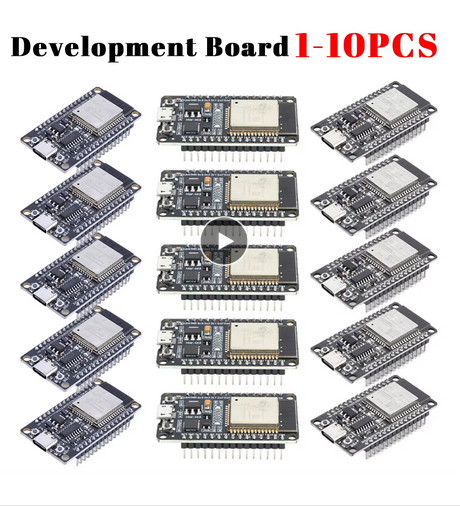
\includegraphics[width=\textwidth]{img/hw_esp32.png}
\caption{ESP32 DevKit V1, usado como puente BLE y futuro puente LIN.}
\label{fig:hw_esp32}
\end{subfigure}
\hfill
\begin{subfigure}[b]{0.3\textwidth}
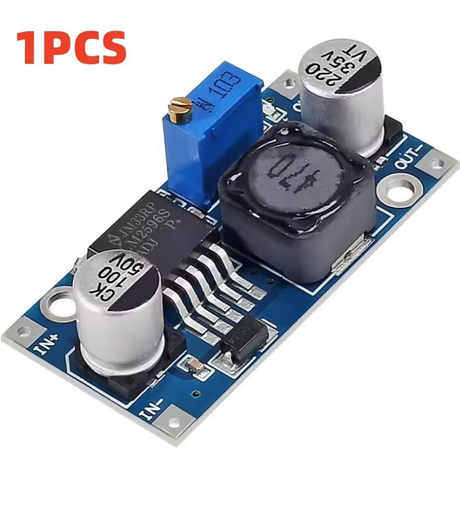
\includegraphics[width=\textwidth]{img/hw_lm2596.png}
\caption{Módulo reductor LM2596 para alimentación del ESP32 desde el bus LIN (12V a 5V).}
\label{fig:hw_lm2596}
\end{subfigure}
\hfill
\begin{subfigure}[b]{0.3\textwidth}
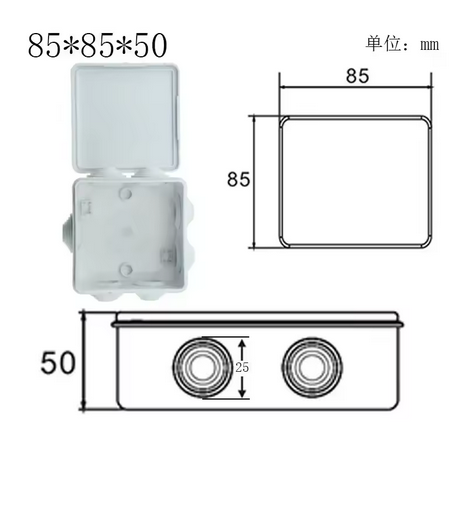
\includegraphics[width=\textwidth]{img/hw_psu_case.png}
\caption{Caja estanca ABS para la fuente de alimentación del sistema HVAC.}
\label{fig:hw_psu_case}
\end{subfigure}
\caption{Componentes hardware del subsistema HVAC: ESP32, regulador de voltaje y caja de protección.}
\label{fig:hw_hvac_components}
\end{figure}

\section{Tabla Comparativa de Alternativas Consideradas}

Para cada componente del software, se evaluaron múltiples alternativas antes de seleccionar la solución final. La Tabla~\ref{tab:alternativas} resume las principales decisiones y su justificación:

\begin{table}[h]
\centering
\footnotesize
\begin{tabular}{|p{2.5cm}|p{2.2cm}|p{2.5cm}|p{3.8cm}|p{3cm}|}
\hline
\textbf{Componente} & \textbf{Seleccionado} & \textbf{Alternativas} & \textbf{Motivo de la elección} & \textbf{Alternativa descartada por} \\
\hline
Inferencia LLM & Ollama & llama.cpp, localAI, GPT4All & Ecosistema maduro, soporte nativo de GPU, API REST estándar~\cite{hui_qwen25_coder_2024} & llama.cpp requiere compilación manual; LocalAI inestable con modelos pequeños \\
\hline
Clasificador ligero & qwen2.5-coder:1.5b & phi-2, gemma-2b, tinyllama & Mejor relación precisión/velocidad en español; soporte multilingüe nativo & phi-2 optimizado para inglés; gemma-2b requiere más VRAM \\
\hline
Razonador & qwen2.5-coder:7b & llama3.2-8b, mistral-7b, zephyr-7b & Similar a 1.5B; consistencia entre niveles del router & llama3.2 necesita más contexto; mistral falla en estructuras JSON \\
\hline
Embeddings & bge-m3 & all-MiniLM-L6-v2, e5-mistral, jina-embeddings & Multilingüe (español+inglés), eficiente en RAM (1.5 GB)~\cite{bge_m3} & all-MiniLM: solo inglés; e5-mistral: demasiado pesado (7B) \\
\hline
BLE Python & bleak & bluepy, pygattlib, gattlib & Async nativo, multiplataforma, mantenimiento activo~\cite{bleak} & bluepy: solo Linux, no async; pygattlib: obsoleto \\
\hline
Tuya local & tinytuya & pytuya, tuyapi, tinyTuya-RF & Soporte protocolo 3.5, activo, documentación clara~\cite{tinytuya} & pytuya: sin mantenimiento; tuyapi: requiere nube \\
\hline
Framework agentes & OpenClaw & Hermes, AutoGPT, n8n & Ligero, canales Telegram+web nativos, Node.js~\cite{openclaw} & Hermes: inmaduro; AutoGPT: sobreingeniería; n8n: no agentes \\
\hline
\end{tabular}
\caption{Comparativa de alternativas tecnológicas consideradas para cada componente del sistema.}
\label{tab:alternativas}
\end{table}

\section{Software y Librerías}

\begin{itemize}
    \item \textbf{Ubuntu Server 24.04 LTS (Noble Numbat):} Sistema operativo del servidor de orquestación. Distribución \textit{headless} con soporte extendido de 5 años.
    \item \textbf{OpenClaw (npm):} \textit{Framework} agéntico para la orquestación de modelos de lenguaje. \textit{Gateway} Node.js con canales nativos (Telegram, \textit{dashboard} web).
    \item \textbf{Ollama:} Servidor de inferencia local para modelos de lenguaje.
    \item \textbf{Python 3.12:} Lenguaje principal del servidor de microservicios (Model Router, Sensor Daemon, Comfort Advisor).
    \item \textbf{C++20:} Lenguaje del firmware del ESP32 (pendiente de implementar).
    \item \textbf{tinytuya:} Librería Python para el control local de dispositivos Tuya.
    \item \textbf{bleak:} Librería Python para comunicación BLE asíncrona.
    \item \textbf{SQLite:} Motor de base de datos relacional embebido (pendiente de implementar).
    \item \textbf{Git / GitHub:} Control de versiones y repositorio del proyecto.
    \item \textbf{\LaTeX:} Sistema de composición tipográfica para la redacción de la memoria.
\end{itemize}

\section{Dependencias de Red}

El ecosistema completo opera sobre un router \textbf{TP-Link TL-MR6400} en configuración \textit{air-gapped}:
\begin{itemize}
    \item Subred: \texttt{192.168.1.0/24}
    \item \textsf{Sin Internet} (ranura SIM rota)
    \item Conexión del servidor por Ethernet dedicada (puerto LAN, no LAN/WAN)
    \item Conexión del portátil y dispositivos Tuya por Wi-Fi 2.4 GHz
    \item Conexión BLE directa para sensores Xiaomi y ventilador FanLamp
\end{itemize}
